% answers.tex —— 2023 年·全国乙卷·文科 · 参考答案与详细解析片段
% 由 tools/generate_projects.py 依来源总账自 2023/2023_数学真题_全国乙文_试题.md + 2023/2023_数学真题_全国乙文_解析正文.md + 2023/2023_数学真题_全国乙文_答案要点.md 生成，勿手改（改源 MD 后重跑）


\begin{gktip}
以下解答均为本库依据固定原卷作出的独立推导，\textbf{非官方答案}，并经另一角色逐题盲核。第 3 题的初稿 \texttt{U} 已依据原卷三视图复核并裁定为 30；第 22 题初稿的值域下界已复算修正为 0。
\end{gktip}

\gkpart{一、单选题}

\begin{answer}
\gksolhead{1}{}

\textbf{题目}：

$|2+\mathrm i^2+2\mathrm i^3|=$\mbox{（　　）}

\begin{gkopts}(4)
\task A．$1$
\task B．$2$
\task C．$\sqrt5$
\task D．$5$
\end{gkopts}

\Needspace{4\baselineskip}
\textbf{解析}

\Needspace{5\baselineskip}
因为 $\mathrm i^2=-1$、$\mathrm i^3=-\mathrm i$，所以

\nopagebreak[4]
\[
|2+\mathrm i^2+2\mathrm i^3|=|1-2\mathrm i|=\sqrt5.
\]

答案：C。

\gkanswer{答案：C（$\sqrt5$）}

\end{answer}
\begin{answer}
\gksolhead{2}{}

\textbf{题目}：

设全集 $U=\{0,1,2,4,6,8\}$，集合 $M=\{0,4,6\}$，$N=\{0,1,6\}$，则 $M\cup\complement_U N=$\mbox{（　　）}

\begin{gkopts}(4)
\task A．$\{0,2,4,6,8\}$
\task B．$\{0,1,4,6,8\}$
\task C．$\{1,2,4,6,8\}$
\task D．$U$
\end{gkopts}

\Needspace{4\baselineskip}
\textbf{解析}

\Needspace{5\baselineskip}
在全集 $U$ 中，$\complement_U N=\{2,4,8\}$，故

\nopagebreak[4]
\[
M\cup\complement_U N=\{0,4,6\}\cup\{2,4,8\}=\{0,2,4,6,8\}.
\]

答案：A。

\gkanswer{答案：A（$\{0,2,4,6,8\}$）}

\end{answer}
\begin{answer}
\gksolhead{3}{}

\textbf{题目}：

如图，网格纸上绘制的是一个零件的三视图，网格小正方形的边长为 $1$，则该零件的表面积为\mbox{（　　）}
\nopagebreak[4]
\begin{center}\begin{tikzpicture}[x=0.42cm,y=0.42cm,line cap=round,line join=round]
  % 左上视图：6×5 网格；原卷粗线轮廓及横线
  \foreach \x in {0,...,6} {\draw[black!35,line width=0.25pt] (\x,0)--(\x,5);}
  \foreach \y in {0,...,5} {\draw[black!35,line width=0.25pt] (0,\y)--(6,\y);}
  \draw[line width=0.85pt] (2,1) rectangle (4,4);
  \draw[line width=0.85pt] (2,3)--(4,3);

  % 右上视图：6×5 网格；两级台阶轮廓
  \begin{scope}[xshift=7cm]
    \foreach \x in {0,...,6} {\draw[black!35,line width=0.25pt] (\x,0)--(\x,5);}
    \foreach \y in {0,...,5} {\draw[black!35,line width=0.25pt] (0,\y)--(6,\y);}
    \draw[line width=0.85pt] (2,1)--(3,1)--(3,2)--(4,2)--(4,4)--(2,4)--cycle;
  \end{scope}

  % 下方视图：6×5 网格；2×2 粗线矩形
  \begin{scope}[yshift=-6cm]
    \foreach \x in {0,...,6} {\draw[black!35,line width=0.25pt] (\x,0)--(\x,5);}
    \foreach \y in {0,...,5} {\draw[black!35,line width=0.25pt] (0,\y)--(6,\y);}
    \draw[line width=0.85pt] (2,1) rectangle (4,3);
  \end{scope}
\end{tikzpicture}
\end{center}
\nopagebreak[4]
\begin{gkopts}(4)
\task A．$24$
\task B．$26$
\task C．$28$
\task D．$30$
\end{gkopts}

\Needspace{4\baselineskip}
\textbf{解析}

\Needspace{5\baselineskip}
答案：D（$30$）。原卷三视图显示，该零件由一个 $2\times2\times2$ 长方体和其上叠放的 $2\times1\times1$ 长方体组成；左上视图的内横线在外框上边向下第一格，右上视图显示相应的一格高差台阶，左下视图给出 $2\times2$ 占地。两个长方体的表面积分别为 $24$ 和 $10$，共用面积为 $2$ 的面被重复计算一次，故

\nopagebreak[4]
\[
S=24+10-2\cdot2=30.
\]

\gkanswer{答案：D（$30$）}

\end{answer}
\begin{answer}
\gksolhead{4}{}

\textbf{题目}：

记 $\triangle ABC$ 的内角 $A$，$B$，$C$ 的对边分别为 $a$，$b$，$c$，若 $a\cos B-b\cos A=c$，且 $C=\dfrac\pi5$，则 $B=$\mbox{（　　）}

\begin{gkopts}(2)
\task A．$\dfrac\pi{10}$
\task B．$\dfrac\pi5$
\task C．$\dfrac{3\pi}{10}$
\task D．$\dfrac{2\pi}5$
\end{gkopts}

\Needspace{4\baselineskip}
\textbf{解析}

\Needspace{5\baselineskip}
由正弦定理，存在 $R>0$ 使 $a=2R\sin A$、$b=2R\sin B$、$c=2R\sin C$。原条件化为

\nopagebreak[4]
\[
\sin A\cos B-\sin B\cos A=\sin C,
\]

即 $\sin(A-B)=\sin C=\sin(A+B)$。由于 $A,B>0$ 且 $A+B=\pi-C=4\pi/5$，非退化解为 $A-B=\pi-(A+B)$，所以 $A=\pi/2$、$B=3\pi/10$。

答案：C。

\gkanswer{答案：C（$B=\dfrac{3\pi}{10}$）}

\end{answer}
\begin{answer}
\gksolhead{5}{}

\textbf{题目}：

已知 $f(x)=\dfrac{xe^x}{e^{ax}-1}$ 是偶函数，则 $a=$\mbox{（　　）}

\begin{gkopts}(4)
\task A．$-2$
\task B．$-1$
\task C．$1$
\task D．$2$
\end{gkopts}

\Needspace{4\baselineskip}
\textbf{解析}

\Needspace{5\baselineskip}
对非零且分母有定义的 $x$，

\nopagebreak[4]
\[
f(-x)=\frac{-xe^{-x}}{e^{-ax}-1}
=\frac{xe^{(a-1)x}}{e^{ax}-1}.
\]

令其等于 $f(x)=xe^x/(e^{ax}-1)$，恒等成立要求 $a-1=1$，故 $a=2$。

答案：D。

\gkanswer{答案：D（$a=2$）}

\end{answer}
\begin{answer}
\gksolhead{6}{}

\textbf{题目}：

已知正方形 $ABCD$ 的边长为 $2$，$E$ 为 $AB$ 的中点，则 $\overrightarrow{EC}\cdot\overrightarrow{ED}=$\mbox{（　　）}

\begin{gkopts}(4)
\task A．$\sqrt5$
\task B．$3$
\task C．$2\sqrt5$
\task D．$5$
\end{gkopts}

\Needspace{4\baselineskip}
\textbf{解析}

\Needspace{5\baselineskip}
取 $A=(0,0),B=(2,0),C=(2,2),D=(0,2)$，则 $E=(1,0)$。于是 $\overrightarrow{EC}=(1,2)$、$\overrightarrow{ED}=(-1,2)$，点积为

\nopagebreak[4]
\[
\overrightarrow{EC}\cdot\overrightarrow{ED}=1\cdot(-1)+2\cdot2=3.
\]

答案：B。

\gkanswer{答案：B（$3$）}

\end{answer}
\begin{answer}
\gksolhead{7}{}

\textbf{题目}：

设 $O$ 为平面直角坐标系的坐标原点，在区域 $\{(x,y)\mid 1\leqslant x^2+y^2\leqslant4\}$ 内随机取一点，记该点为 $A$，则直线 $OA$ 的倾斜角不大于 $\dfrac\pi4$ 的概率为\mbox{（　　）}

\begin{gkopts}(4)
\task A．$\dfrac18$
\task B．$\dfrac16$
\task C．$\dfrac14$
\task D．$\dfrac12$
\end{gkopts}

\Needspace{4\baselineskip}
\textbf{解析}

环域关于原点旋转对称，半径取值不影响直线方向。直线的倾斜角按模 $\pi$ 计，$[0,\pi/4]$ 占 $[0,\pi)$ 的 $1/4$，所以所求概率为 $1/4$。

答案：C。

\gkanswer{答案：C（$\dfrac14$）}

\end{answer}
\begin{answer}
\gksolhead{8}{}

\textbf{题目}：

若函数 $f(x)=x^3+ax+2$ 存在 $3$ 个零点，则 $a$ 的取值范围是\mbox{（　　）}

\begin{gkopts}(4)
\task A．$(-\infty,-2)$
\task B．$(-\infty,-3)$
\task C．$(-4,-1)$
\task D．$(-3,0)$
\end{gkopts}

\Needspace{4\baselineskip}
\textbf{解析}

\Needspace{5\baselineskip}
若 $f(x)=x^3+ax+2$ 有三个不同实零点，必须有 $a<0$，并且两个驻点处函数值异号。令 $r=\sqrt{-a/3}>0$，驻点为 $\pm r$，且

\nopagebreak[4]
\[
f(-r)=2+2r^3>0,\qquad f(r)=2-2r^3.
\]

要求 $f(r)<0$，即 $r>1$，等价于 $a<-3$。

答案：B。

\gkanswer{答案：B（$a<-3$）}

\end{answer}
\begin{answer}
\gksolhead{9}{}

\textbf{题目}：

某学校举办作文比赛，共设 $6$ 个主题，每位参赛同学从中随机抽取一个主题准备作文．则甲、乙两位参赛同学抽到不同主题的概率为\mbox{（　　）}

\begin{gkopts}(4)
\task A．$\dfrac56$
\task B．$\dfrac23$
\task C．$\dfrac12$
\task D．$\dfrac13$
\end{gkopts}

\Needspace{4\baselineskip}
\textbf{解析}

甲、乙各自独立且等可能地从 $6$ 个主题中选一个。两人选到相同主题的概率为 $1/6$，故选到不同主题的概率为 $1-1/6=5/6$。

答案：A。

\gkanswer{答案：A（$\dfrac56$）}

\end{answer}
\begin{answer}
\gksolhead{10}{}

\textbf{题目}：

已知函数 $f(x)=\sin(\omega x+\varphi)$ 在区间 $\left(\dfrac\pi6,\dfrac{2\pi}3\right)$ 单调递增，直线 $x=\dfrac\pi6$ 和 $x=\dfrac{2\pi}3$ 为函数 $y=f(x)$ 的图象的两条对称轴，则 $f\left(-\dfrac{5\pi}{12}\right)=$\mbox{（　　）}

\begin{gkopts}(2)
\task A．$-\dfrac{\sqrt3}{2}$
\task B．$-\dfrac12$
\task C．$\dfrac12$
\task D．$\dfrac{\sqrt3}{2}$
\end{gkopts}

\Needspace{4\baselineskip}
\textbf{解析}

\Needspace{5\baselineskip}
正弦图象相邻对称轴相距 $\pi/|\omega|$。严格递增区间中不能再有极值轴，所以给定两轴相邻，轴距为 $\pi/2$，得 $|\omega|=2$。左端是极小值，故 $\omega\pi/6+\varphi\equiv-\pi/2\pmod{2\pi}$。计算点 $-5\pi/12$ 与左端的横坐标差为 $-7\pi/12$，于是相位差为 $-7\omega\pi/12$。若 $\omega=2$，该点相位等价于 $-5\pi/3$；若 $\omega=-2$，该点相位等价于 $2\pi/3$。两种情况下函数值均为 $\sqrt3/2$：

\nopagebreak[4]
\[
f\left(-\frac{5\pi}{12}\right)=\frac{\sqrt3}{2}.
\]

答案：D。

\gkanswer{答案：D（$\dfrac{\sqrt3}{2}$）}

\end{answer}
\begin{answer}
\gksolhead{11}{}

\textbf{题目}：

已知 $x,y$ 满足 $x^2+y^2-4x-2y-4=0$，则 $x-y$ 的最大值是\mbox{（　　）}

\begin{gkopts}(2)
\task A．$1+\dfrac{3\sqrt2}{2}$
\task B．$4$
\task C．$1+3\sqrt2$
\task D．$7$
\end{gkopts}

\Needspace{4\baselineskip}
\textbf{解析}

\Needspace{5\baselineskip}
配方得 $(x-2)^2+(y-1)^2=9$，即圆心 $(2,1)$、半径 $3$。线性函数 $x-y$ 的最大值等于圆心处的值加半径乘系数向量模：

\nopagebreak[4]
\[
\max(x-y)=2-1+3\sqrt{1^2+(-1)^2}=1+3\sqrt2.
\]

答案：C。

\gkanswer{答案：C（$1+3\sqrt2$）}

\end{answer}
\begin{answer}
\gksolhead{12}{}

\textbf{题目}：

设 $A,B$ 为双曲线 $x^2-\dfrac{y^2}{9}=1$ 上两点，下列四个点中，可以为线段 $AB$ 中点的是\mbox{（　　）}

\begin{gkopts}(4)
\task A．$(1,1)$
\task B．$(-1,2)$
\task C．$(1,3)$
\task D．$(-1,-4)$
\end{gkopts}

\Needspace{4\baselineskip}
\textbf{解析}

\Needspace{5\baselineskip}
设候选中点为 $M=(h,k)$，半弦向量为 $(u,v)$，则两端点是 $M\pm(u,v)$。使它们都在双曲线上，需满足

\nopagebreak[4]
\[
hu-\frac{kv}{9}=0,\qquad
u^2-\frac{v^2}{9}=1-h^2+\frac{k^2}{9}.
\]

\Needspace{5\baselineskip}
对 A、B 两点，$h^2-k^2/9$ 分别为 $8/9,5/9$；对 C 点该值为 $0$。由第一式代入第二式时，左侧非正而右侧为正，均不可能。对 D 点 $M=(-1,-4)$，取

\nopagebreak[4]
\[
u=\frac{16}{3\sqrt7},\qquad v=\frac{12}{\sqrt7},
\]

两式同时成立，故确有一对不同的双曲线上端点以 D 为中点。

答案：D。

\gkanswer{答案：D（$(-1,-4)$）}

\end{answer}
\gkpart{二、填空题}

\begin{answer}
\gksolhead{13}{}

\textbf{题目}：

已知点 $A(1,\sqrt5)$ 在抛物线 $C:y^2=2px$ 上，则 $A$ 到 $C$ 的准线的距离为 \gkblank{}．

\Needspace{4\baselineskip}
\textbf{解析}

\Needspace{5\baselineskip}
将 $A(1,\sqrt5)$ 代入 $y^2=2px$，得 $5=2p$，故 $p=5/2$。准线为 $x=-p/2=-5/4$，点 $A$ 到准线的距离为

\nopagebreak[4]
\[
1+\frac54=\frac94.
\]

\gkanswer{答案：$\dfrac94$}

\end{answer}
\begin{answer}
\gksolhead{14}{}

\textbf{题目}：

若 $\theta\in\left(0,\dfrac\pi2\right)$，$\tan\theta=\dfrac13$，则 $\sin\theta-\cos\theta=$ \gkblank{}．

\Needspace{4\baselineskip}
\textbf{解析}

\Needspace{5\baselineskip}
由 $\tan\theta=1/3$ 且 $0<\theta<\pi/2$，有 $\sin\theta=1/\sqrt{10}$、$\cos\theta=3/\sqrt{10}$，所以

\nopagebreak[4]
\[
\sin\theta-\cos\theta=-\frac2{\sqrt{10}}.
\]

\gkanswer{答案：$-\dfrac{2}{\sqrt{10}}$}

\end{answer}
\begin{answer}
\gksolhead{15}{}

\textbf{题目}：

\Needspace{5\baselineskip}
若 $x,y$ 满足约束条件

\nopagebreak[4]
\[
\begin{cases}
x-3y\leqslant-1,\\
x+2y\leqslant9,\\
3x+y\geqslant7,
\end{cases}
\]

则 $z=2x-y$ 的最大值为 \gkblank{}．

\Needspace{4\baselineskip}
\textbf{解析}

三条边界线两两相交得到可行域顶点 $(2,1)$、$(5,2)$、$(1,4)$。目标函数 $z=2x-y$ 在三点的值分别为 $3,8,-2$，所以最大值为 $8$。

\gkanswer{答案：$8$}

\end{answer}
\begin{answer}
\gksolhead{16}{}

\textbf{题目}：

已知点 $S,A,B,C$ 均在半径为 $2$ 的球面上，$\triangle ABC$ 是边长为 $3$ 的等边三角形，$SA\perp$ 平面 $ABC$，则 $SA=$ \gkblank{}．

\Needspace{4\baselineskip}
\textbf{解析}

底面等边三角形的外接圆半径为 $3/\sqrt3=\sqrt3$。设 $A=(0,0,0)$、$S=(0,0,h)$，平面 $ABC$ 为 $z=0$。球心在底面外接圆心的法线上，到平面距离记为 $c$。由球半径为 $2$，有 $3+c^2=4$，故 $|c|=1$。球心到 $A,S$ 等距，比较两距离平方得 $c^2=(c-h)^2$；非退化情形下 $h=2c$，所以 $SA=|h|=2$。

\gkanswer{答案：$2$}

\end{answer}
\gkpart{三、解答题}

\begin{answer}
\gksolhead{17}{}

\textbf{题目}：

某厂为比较甲、乙两种工艺对橡胶产品伸缩率的处理效应，进行 $10$ 次配对试验，每次配对试验选用材质相同的两个橡胶产品，随机地选其中一个用甲工艺处理，另一个用乙工艺处理，测量处理后的橡胶产品的伸缩率．甲、乙两种工艺处理后的橡胶产品的伸缩率分别记为 $x_i,y_i$（$i=1,2,\cdots,10$）．试验结果如下：

\begin{center}
\begingroup\setlength{\tabcolsep}{4pt}
\begin{tabular}{crrrrrrrrrr}
\toprule
试验序号 $i$ & 1 & 2 & 3 & 4 & 5 & 6 & 7 & 8 & 9 & 10 \\
\midrule
伸缩率 $x_i$ & 545 & 533 & 551 & 522 & 575 & 544 & 541 & 568 & 596 & 548 \\
伸缩率 $y_i$ & 536 & 527 & 543 & 530 & 560 & 533 & 522 & 550 & 576 & 536 \\
\bottomrule
\end{tabular}
\endgroup
\end{center}

记 $z_i=x_i-y_i$（$i=1,2,\cdots,10$），记 $z_1,z_2,\cdots,z_{10}$ 的样本平均数为 $\bar z$，样本方差为 $s^2$．

（1） 求 $\bar z,s^2$；

（2） 判断甲工艺处理后的橡胶产品的伸缩率较乙工艺处理后的橡胶产品的伸缩率是否有显著提高（如果 $\bar z\geqslant2\sqrt{\dfrac{s^2}{10}}$，则认为甲工艺处理后的橡胶产品的伸缩率较乙工艺处理后的橡胶产品的伸缩率有显著提高，否则不认为有显著提高）．

\Needspace{4\baselineskip}
\textbf{解析}

\gksubpart{(1) 求样本平均数和方差}

\Needspace{5\baselineskip}
逐项作差得

\nopagebreak[4]
\[
(z_1,\ldots,z_{10})=(9,6,8,-8,15,11,19,18,20,12),\qquad \sum z_i=110.
\]

\Needspace{5\baselineskip}
因此 $\bar z=11$。离均差平方和为

\nopagebreak[4]
\[
(-2)^2+(-5)^2+(-3)^2+(-19)^2+4^2+0^2+8^2+7^2+9^2+1^2=610,
\]

按高中统计中样本方差的定义 $s^2=\dfrac1{10}\sum_{i=1}^{10}(z_i-\bar z)^2$，得 $s^2=61$。

\gksubpart{(2) 判断是否显著提高}

\Needspace{5\baselineskip}
检验阈值为

\nopagebreak[4]
\[
2\sqrt{\frac{s^2}{10}}=2\sqrt{\frac{61}{10}}<11=\bar z,
\]

故按题设规则，认为甲工艺处理后的伸缩率有显著提高。

\gkanswer{答案（1）：$\bar z=11,\ s^2=61$}

\gkanswer{答案（2）：有显著提高。}

\end{answer}
\begin{answer}
\gksolhead{18}{}

\textbf{题目}：

记 $S_n$ 为等差数列 $\{a_n\}$ 的前 $n$ 项和．已知 $a_2=11$，$S_{10}=40$．

（1） 求 $\{a_n\}$ 的通项公式；

（2） 求数列 $\{|a_n|\}$ 的前 $n$ 项和 $T_n$．

\Needspace{4\baselineskip}
\textbf{解析}

\gksubpart{(1) 求等差数列通项}

\Needspace{5\baselineskip}
设等差数列首项为 $a_1$、公差为 $d$。由条件

\nopagebreak[4]
\[
a_1+d=11,\qquad 5(2a_1+9d)=40,
\]

\Needspace{5\baselineskip}
解得 $a_1=13,d=-2$，于是

\nopagebreak[4]
\[
a_n=13-2(n-1)=15-2n.
\]

\gksubpart{(2) 求绝对值数列前 $n$ 项和}

\Needspace{5\baselineskip}
当 $1\leqslant n\leqslant7$ 时，前 $n$ 项均为正，

\nopagebreak[4]
\[
T_n=\sum_{k=1}^n(15-2k)=n(14-n).
\]

\Needspace{5\baselineskip}
当 $n\geqslant8$ 时，前七项绝对值之和为 $49$，且 $k\geqslant8$ 时 $|a_k|=2k-15$，所以

\nopagebreak[4]
\[
T_n=49+\sum_{k=8}^n(2k-15)=n^2-14n+98.
\]

\gkanswer{答案（1）：$a_n=15-2n$}

\gkanswer{答案（2）：$T_n=n(14-n)$（$1\leqslant n\leqslant7$）；$T_n=n^2-14n+98$（$n\geqslant8$）。}

\end{answer}
\begin{answer}
\gksolhead{19}{}

\textbf{题目}：

如图，在三棱锥 $P-ABC$ 中，$AB\perp BC$，$AB=2$，$BC=2\sqrt2$，$PB=PC=\sqrt6$，$BP,AP,BC$ 的中点分别为 $D,E,O$，点 $F$ 在 $AC$ 上，$BF\perp AO$．
\nopagebreak[4]
\begin{center}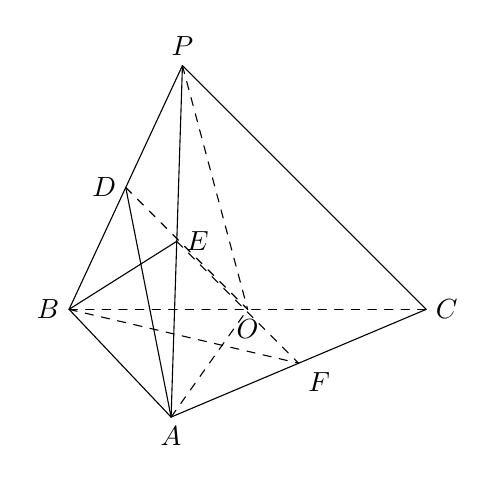
\begin{tikzpicture}[x=0.72cm,y=0.72cm,line cap=round,line join=round]
  \coordinate (P) at (2.0,6.6);
  \coordinate (A) at (1.8,0.4);
  \coordinate (B) at (0,2.3);
  \coordinate (C) at (6.3,2.3);
  \coordinate (D) at (1.0,4.45);
  \coordinate (E) at (1.9,3.5);
  \coordinate (O) at (3.15,2.3);
  \coordinate (F) at (4.05,1.35);

  % 三棱锥外棱及面内可见线
  \draw (P)--(B)--(A)--(C)--(P);
  \draw (P)--(A);
  \draw (D)--(A);
  \draw (B)--(E);
  \draw[dashed] (E)--(F);

  % 原图中的遮挡线
  \draw[dashed] (B)--(C);
  \draw[dashed] (P)--(O);
  \draw[dashed] (D)--(O);
  \draw[dashed] (A)--(O);
  \draw[dashed] (B)--(F);

  \node[above] at (P) {$P$};
  \node[below] at (A) {$A$};
  \node[left] at (B) {$B$};
  \node[right] at (C) {$C$};
  \node[left] at (D) {$D$};
  \node[right] at (E) {$E$};
  \node[below] at (O) {$O$};
  \node[below right] at (F) {$F$};
\end{tikzpicture}
\end{center}
\nopagebreak[4]
（1） 证明：$EF\parallel$ 平面 $ADO$；

（2） 若 $\angle POF=120^\circ$，求三棱锥 $P-ABC$ 的体积．

\Needspace{4\baselineskip}
\textbf{解析}

\gksubpart{(1) 证明线面平行}

\Needspace{5\baselineskip}
取

\nopagebreak[4]
\[
B=(0,0,0),\quad A=(2,0,0),\quad C=(0,2\sqrt2,0),\quad
P=(u,\sqrt2,v).
\]

\Needspace{5\baselineskip}
由 $PB=PC=\sqrt6$ 得 $u^2+v^2=4$。设 $F=A+t(C-A)=(2-2t,2\sqrt2t,0)$。因 $AO$ 的方向向量为 $(-2,\sqrt2,0)$，条件 $BF\perp AO$ 给出

\nopagebreak[4]
\[
(-2,\sqrt2,0)\cdot(2-2t,2\sqrt2t,0)=-4+8t=0,
\]

故 $t=1/2$，$F$ 是 $AC$ 的中点。$E$ 是 $AP$ 的中点，因此在三角形 $APC$ 中 $EF\parallel PC$。

\Needspace{5\baselineskip}
再证 $PC\parallel\text{\text{平面} }ADO$。平面内两方向向量可取

\nopagebreak[4]
\[
\overrightarrow{AD}=\left(\frac u2-2,\frac{\sqrt2}2,\frac v2\right),\qquad
\overrightarrow{AO}=(-2,\sqrt2,0).
\]

\Needspace{5\baselineskip}
其法向量可取 $\boldsymbol n=(-v/\sqrt2,-v,(u-2)/\sqrt2)$。而

\nopagebreak[4]
\[
\overrightarrow{PC}=(u,-\sqrt2,v),\qquad \boldsymbol n\cdot\overrightarrow{PC}=0,
\]

故 $PC$ 的方向平行平面 $ADO$，进而 $EF\parallel\text{\text{平面} }ADO$。

\gksubpart{(2) 求三棱锥体积}

\Needspace{5\baselineskip}
由 $O=(0,\sqrt2,0)$、$F=(1,\sqrt2,0)$，有 $\overrightarrow{OF}=(1,0,0)$、$|OF|=1$，又 $|OP|=2$。所以

\nopagebreak[4]
\[
\cos\angle POF=\frac{\overrightarrow{OP}\cdot\overrightarrow{OF}}{|OP||OF|}=\frac u2=-\frac12,
\]

\Needspace{5\baselineskip}
从而 $u=-1$、$|v|=\sqrt3$。底面面积为 $\frac12\cdot2\cdot2\sqrt2=2\sqrt2$，棱锥高为 $|v|$，体积

\nopagebreak[4]
\[
V=\frac13\cdot2\sqrt2\cdot\sqrt3=\frac{2\sqrt6}{3}.
\]

\gkanswer{答案（1）：见解析版}

\gkanswer{答案（2）：$V=\dfrac{2\sqrt6}{3}$}

\end{answer}
\begin{answer}
\gksolhead{20}{}

\textbf{题目}：

已知函数 $f(x)=\left(\dfrac1x+a\right)\ln(1+x)$．

（1） 当 $a=-1$ 时，求曲线 $y=f(x)$ 在点 $(1,f(1))$ 处的切线方程；

（2） 若 $f(x)$ 在 $(0,+\infty)$ 单调递增，求 $a$ 的取值范围．

\Needspace{4\baselineskip}
\textbf{解析}

\gksubpart{(1) 求切线方程}

\Needspace{5\baselineskip}
（1）当 $a=-1$ 时，$f(x)=(1/x-1)\ln(1+x)$，故 $f(1)=0$。求导得

\nopagebreak[4]
\[
f'(x)=-\frac{\ln(1+x)}{x^2}+\frac{1/x-1}{1+x},
\]

\Needspace{5\baselineskip}
于是 $f'(1)=-\ln2$。切线为

\nopagebreak[4]
\[
y=-\ln2(x-1)=(1-x)\ln2.
\]

\gksubpart{(2) 求参数范围}

\Needspace{5\baselineskip}
（2）对 $x>0$，

\nopagebreak[4]
\[
f'(x)=\frac{a x^2+x-(1+x)\ln(1+x)}{x^2(1+x)}.
\]

\Needspace{5\baselineskip}
令 $G(x)=(1+x)\ln(1+x)-x$。有 $G(0)=0$ 且 $G'(x)=\ln(1+x)<x$，所以 $G(x)<x^2/2$。因此 $a\geqslant1/2$ 时 $f'(x)>0$ 对所有 $x>0$ 成立。若 $a<1/2$，由 $G(x)/x^2\to1/2$（$x\to0^+$），可取充分小的正 $x$ 使 $a<G(x)/x^2$，此时 $f'(x)<0$，不可能在整个区间单调递增。故

\nopagebreak[4]
\[
a\in\left[\frac12,+\infty\right).
\]

\gkanswer{答案（1）：$y=(1-x)\ln2$}

\gkanswer{答案（2）：$a\in[\dfrac12,+\infty)$}

\end{answer}
\begin{answer}
\gksolhead{21}{}

\textbf{题目}：

已知椭圆 $C:\dfrac{y^2}{a^2}+\dfrac{x^2}{b^2}=1$（$a>b>0$）的离心率为 $\dfrac{\sqrt5}{3}$，点 $A(-2,0)$ 在 $C$ 上．

（1） 求 $C$ 的方程；

（2） 过点 $(-2,3)$ 的直线交 $C$ 于 $P,Q$ 两点，直线 $AP,AQ$ 与 $y$ 轴的交点分别为 $M,N$，证明：线段 $MN$ 的中点为定点．

\Needspace{4\baselineskip}
\textbf{解析}

\gksubpart{(1) 求椭圆方程}

\Needspace{5\baselineskip}
（1）椭圆离心率满足 $1-b^2/a^2=5/9$，所以 $b^2/a^2=4/9$。点 $A(-2,0)$ 在椭圆上，得 $b^2=4$，从而 $a^2=9$，方程为

\nopagebreak[4]
\[
\frac{x^2}{4}+\frac{y^2}{9}=1.
\]

\gksubpart{(2) 证明弦中点为定点}

\Needspace{5\baselineskip}
（2）设过 $(-2,3)$ 的非竖直直线斜率为 $k$，则 $y=kx+2k+3$。代入椭圆，交点横坐标 $x_1,x_2$ 是

\nopagebreak[4]
\[
(9+4k^2)x^2+8k(2k+3)x+4(2k+3)^2-36=0
\]

\Needspace{5\baselineskip}
的两根。因此

\nopagebreak[4]
\[
x_1+x_2=-\frac{8k(2k+3)}{9+4k^2},\qquad
x_1x_2=\frac{16k(k+3)}{9+4k^2}.
\]

\Needspace{5\baselineskip}
记直线 $AP,AQ$ 的斜率为 $m_1,m_2$。因为 $A=(-2,0)$，其与 $y$ 轴交点纵坐标分别为 $2m_1,2m_2$。又 $y_i=kx_i+2k+3$，故

\nopagebreak[4]
\[
m_i=\frac{y_i}{x_i+2}=k+\frac3{x_i+2}.
\]

\Needspace{5\baselineskip}
由根和、根积，

\nopagebreak[4]
\[
x_1+x_2+4=\frac{12(3-2k)}{9+4k^2},\qquad
(x_1+2)(x_2+2)=\frac{36}{9+4k^2},
\]

\Needspace{5\baselineskip}
从而

\nopagebreak[4]
\[
m_1+m_2=2k+3\frac{x_1+x_2+4}{(x_1+2)(x_2+2)}=3.
\]

所以 $M,N$ 的纵坐标和恒为 $2m_1+2m_2=6$，其中点的纵坐标恒为 $3$；中点定点为 $(0,3)$。

\gkanswer{答案（1）：$\dfrac{x^2}{4}+\dfrac{y^2}{9}=1$}

\gkanswer{答案（2）：见解析版}

\end{answer}
\begin{answer}
\gksolhead{22}{}

\textbf{题目}：

\Needspace{5\baselineskip}
在直角坐标系 $xOy$ 中，以坐标原点为极点，$x$ 轴正半轴为极轴建立极坐标系，曲线 $C_1$ 的极坐标方程为 $\rho=2\sin\theta\ \left(\dfrac\pi4\leqslant\theta\leqslant\dfrac\pi2\right)$．曲线 $C_2$：

\nopagebreak[4]
\[
\begin{cases}
x=2\cos\alpha,\\
y=2\sin\alpha,
\end{cases}
\qquad(\alpha\text{ \text{为参数，}}\ \dfrac\pi2<\alpha<\pi).
\]

（1） 写出 $C_1$ 的直角坐标方程；

（2） 若直线 $y=x+m$ 既与 $C_1$ 没有公共点，也与 $C_2$ 没有公共点，求 $m$ 的取值范围．

\Needspace{4\baselineskip}
\textbf{解析}

\gksubpart{(1) 化为直角坐标方程}

\Needspace{5\baselineskip}
（1）利用 $x=\rho\cos\theta,y=\rho\sin\theta$，由 $\rho=2\sin\theta$ 得

\nopagebreak[4]
\[
x^2+y^2=2y,\qquad x^2+(y-1)^2=1.
\]

给定角度范围还要求 $x\geqslant0,y\geqslant1$，所以它表示该圆的一段弧。

\gksubpart{(2) 求参数范围}

\Needspace{5\baselineskip}
（2）直线 $y=x+m$ 与曲线有交点等价于相应曲线上 $y-x=m$。在 $C_1$ 上，

\nopagebreak[4]
\[
y-x=2\sin^2\theta-\sin2\theta=2\sin\theta(\sin\theta-\cos\theta),
\]

\Needspace{5\baselineskip}
令 $t=2\theta\in[\pi/2,\pi]$，则 $y-x=1-\cos t-\sin t$，其导数 $\sin t-\cos t>0$，故 $C_1$ 上的值域为 $[0,2]$。在 $C_2$ 上，

\nopagebreak[4]
\[
y-x=2(\sin\alpha-\cos\alpha),\qquad \frac\pi2<\alpha<\pi,
\]

\Needspace{5\baselineskip}
值域为 $(2,2\sqrt2]$。因此直线与 $C_1,C_2$ 均无公共点的条件是

\nopagebreak[4]
\[
m\notin[0,2]\cup(2,2\sqrt2],
\]

\Needspace{5\baselineskip}
即

\nopagebreak[4]
\[
m\in(-\infty,0)\cup(2\sqrt2,+\infty).
\]

\gkanswer{答案（1）：$x^2+y^2=2y$，取题设对应圆弧}

\gkanswer{答案（2）：$m\in(-\infty,0)\cup(2\sqrt2,+\infty)$}

\end{answer}
\begin{answer}
\gksolhead{23}{}

\textbf{题目}：

已知 $f(x)=2|x|+|x-2|$．

（1） 求不等式 $f(x)\leqslant6-x$ 的解集；

\Needspace{5\baselineskip}
（2） 在直角坐标系 $xOy$ 中，求不等式组

\nopagebreak[4]
\[
\begin{cases}
f(x)\leqslant y,\\
x+y-6\leqslant0
\end{cases}
\]

所确定的平面区域的面积．

\Needspace{4\baselineskip}
\textbf{解析}

\gksubpart{(1) 求不等式解集}

（1）分段去绝对值：

\Needspace{5\baselineskip}
当 $x\leqslant0$ 时，$f(x)=2-3x$，不等式化为 $x\geqslant-2$；当 $0\leqslant x\leqslant2$ 时，$f(x)=x+2$，不等式恒成立；当 $x\geqslant2$ 时，$f(x)=3x-2$，不等式要求 $x\leqslant2$。合并得

\nopagebreak[4]
\[
x\in[-2,2].
\]

\gksubpart{(2) 求平面区域面积}

\Needspace{5\baselineskip}
（2）区域上下边界为 $y=f(x)$ 与 $y=6-x$，可行横坐标正是 $[-2,2]$。因此面积为

\nopagebreak[4]
\[
\int_{-2}^0\big[(6-x)-(2-3x)\big]dx+
\int_0^2\big[(6-x)-(x+2)\big]dx
=\int_{-2}^0(4+2x)dx+\int_0^2(4-2x)dx=4+4=8.
\]

\gkanswer{答案（1）：$[-2,2]$}

\gkanswer{答案（2）：$8$}

\end{answer}